\chapter{Introduction}
\label{ch:introduction}

\begin{figure}[H]
\centering
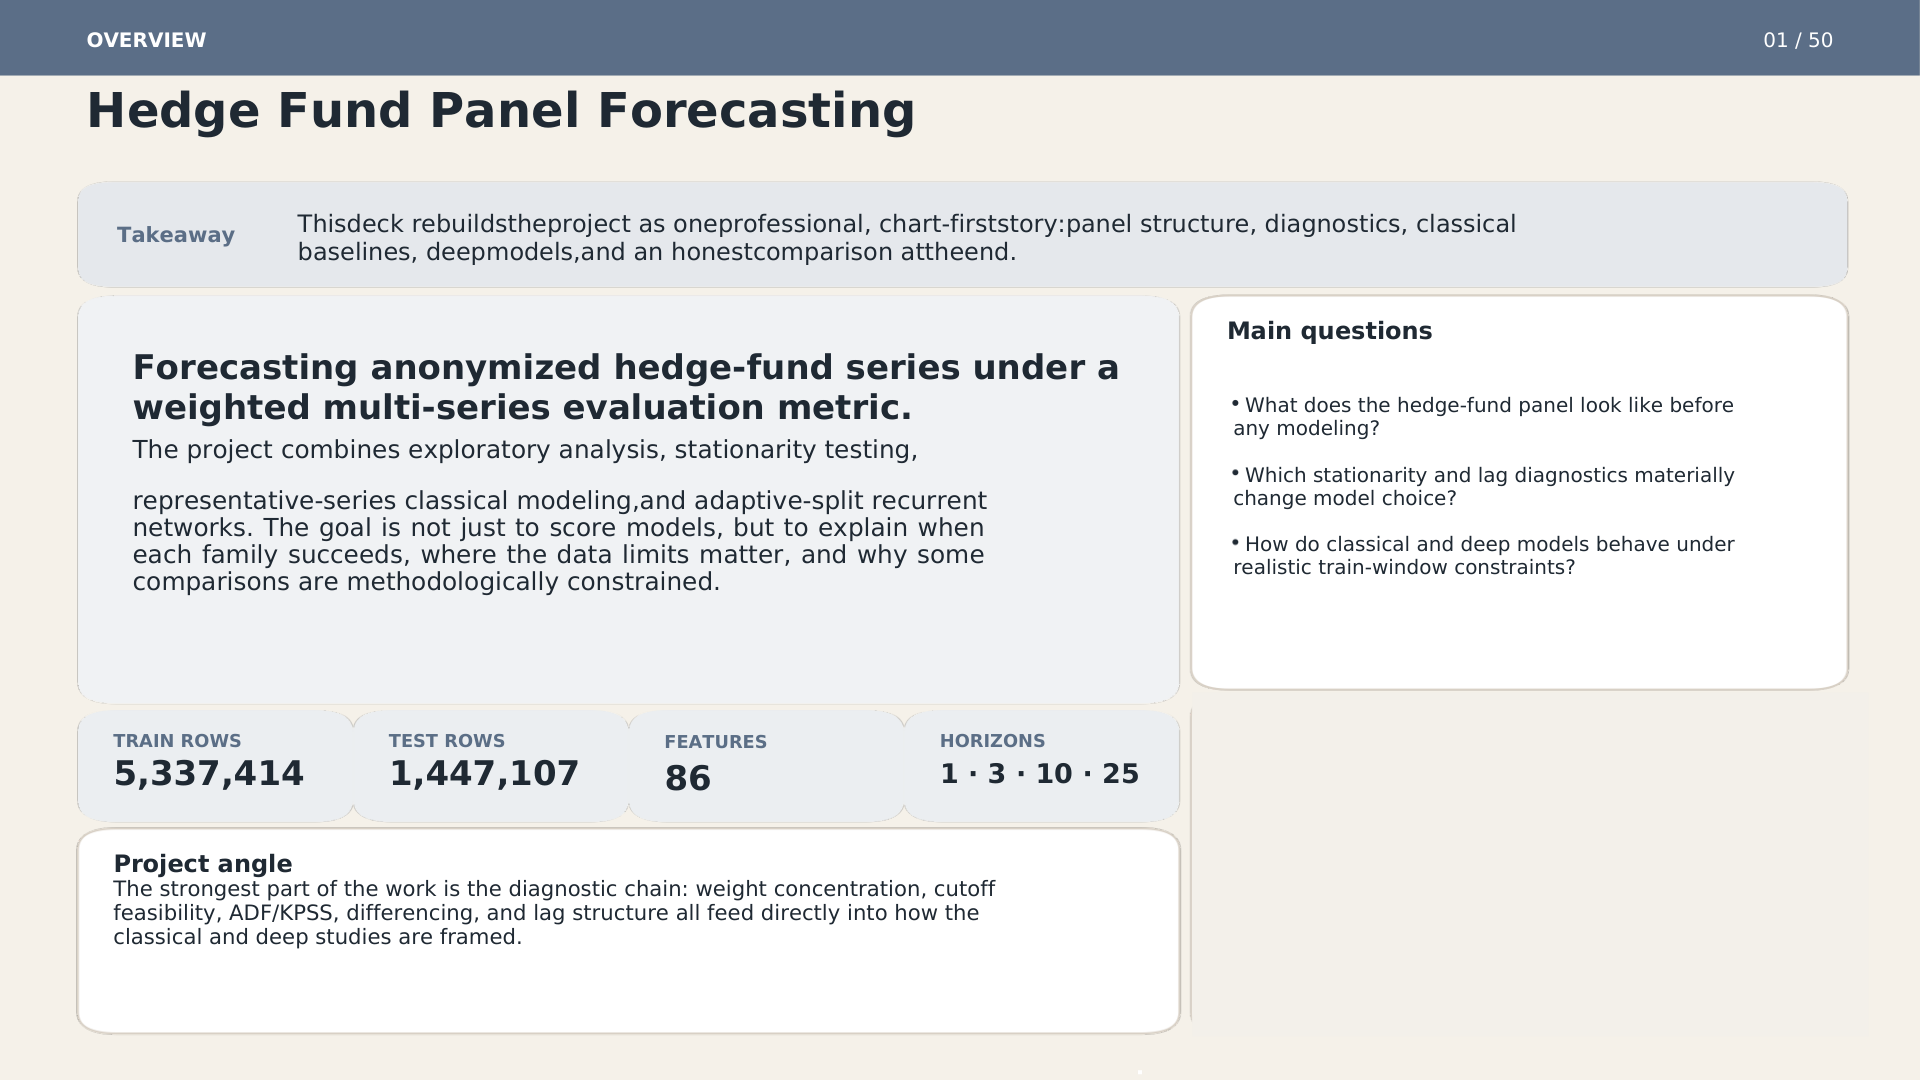
\includegraphics[width=0.95\textwidth]{figures/slide_01.png}
\caption{Project overview: Hedge Fund Panel Forecasting. The project addresses forecasting of 5.3M+ training rows across 86 features and 4 horizons, combining EDA, classical baselines, and deep models.}
\label{fig:overview}
\end{figure}

\section{Motivation and Background}

Time series forecasting lies at the heart of quantitative finance. Hedge funds, asset managers, and proprietary trading desks rely on predictive models to anticipate market movements, optimize portfolio allocation, and manage risk. The ability to forecast financial time series accurately---even marginally---can translate into substantial economic value.

This project addresses the \textbf{Kaggle ``Hedge Fund --- Time Series Forecasting''} competition (competition slug: \texttt{ts-forecasting}), hosted by \emph{A data COMPANY}. The competition ran from January~9, 2026 through April~7, 2026, attracting 3,211 entrants, 1,063 active participants across 982 teams, and 4,127 total submissions. A prize pool of \$10,000 underscored the real-world relevance of the task.

The challenge encapsulates a canonical problem in quantitative research: given a large, anonymized panel of financial time series---each identified by entity codes, sub-categories, and forecast horizons---build models that generalize robustly out-of-sample. The anonymization removes domain shortcuts; success depends entirely on the statistical and machine-learning methodology applied.

\section{Project Objectives}

The objectives of this project are threefold:

\begin{enumerate}[label=(\roman*)]
    \item \textbf{Comprehensive Exploratory Data Analysis (EDA):} Understand the structure, distributional properties, temporal dynamics, and weight distribution of the panel dataset before any modeling.
    \item \textbf{Classical Statistical Modeling:} Establish defensible baselines and univariate benchmarks using AR, MA, ARMA, ARIMA, and SARIMA families, rigorously honoring the stationarity findings from the EDA.
    \item \textbf{Deep Sequence Modeling:} Implement and evaluate recurrent neural network architectures---vanilla RNN, GRU, and LSTM---that can capture nonlinear temporal dependencies the classical models cannot.
\end{enumerate}

\section{Report Structure}

This report is organized as follows:

\begin{itemize}
    \item \textbf{Chapter~\ref{ch:competition}} provides a detailed description of the Kaggle competition: rules, evaluation metric, data schema, and submission format.
    \item \textbf{Chapter~\ref{ch:data}} describes the dataset in depth, including the panel structure, feature space, target variable, weight distribution, and train/test split design.
    \item \textbf{Chapter~\ref{ch:eda}} presents the full exploratory data analysis: missing values, distributional analysis, stationarity testing, autocorrelation structure, cross-correlation analysis, weight concentration, and STL decomposition.
    \item \textbf{Chapter~\ref{ch:classical}} covers the classical modeling pipeline: 41 model specifications across 6 families, the evaluation framework, leaderboard results, per-series winner analysis, and residual diagnostics.
    \item \textbf{Chapter~\ref{ch:deep}} details the deep learning approach: RNN, GRU, and LSTM architectures, the recursive forecasting strategy, adaptive training splits, and hyperparameter choices.
    \item \textbf{Chapter~\ref{ch:results}} synthesizes results across all modeling approaches, comparing classical versus deep learning performance.
    \item \textbf{Chapter~\ref{ch:conclusion}} summarizes key findings, discusses limitations, and outlines directions for future work.
\end{itemize}

\section{Technical Environment}

All experiments were conducted in Python~3.12 using Jupyter notebooks. The core dependencies are:

\begin{table}[H]
\centering
\caption{Core software dependencies.}
\label{tab:dependencies}
\begin{tabular}{ll}
\toprule
\textbf{Library} & \textbf{Purpose} \\
\midrule
NumPy & Numerical computation \\
Pandas & Data manipulation and panel operations \\
Matplotlib / Seaborn & Visualization \\
Statsmodels & Classical time series models (ARIMA, SARIMA, ADF tests) \\
PyTorch & Deep learning (RNN, GRU, LSTM) \\
PyArrow & Parquet file I/O \\
scikit-learn & Preprocessing and utilities \\
\bottomrule
\end{tabular}
\end{table}

The project repository contains three primary notebooks:
\begin{enumerate}
    \item \texttt{01\_eda.ipynb} --- Exploratory Data Analysis
    \item \texttt{02\_classical\_models\_claude.ipynb} --- Classical Statistical Models
    \item \texttt{03\_deep\_sequence\_models\_chosen.ipynb} --- Deep Sequence Models (RNN, GRU, LSTM)
\end{enumerate}


\chapter{Competition Overview}
\label{ch:competition}

\section{Competition Description}

The \textbf{Hedge Fund --- Time Series Forecasting} competition on Kaggle tasks participants with predicting future values of anonymized financial time series. The competition is hosted by \emph{A data COMPANY} and is classified as a \emph{Community Prediction Competition}.

The official description states:
\begin{quote}
\itshape
Participants will receive an integer-indexed time series dataset (\texttt{ts\_index} column), where each record is identified by a code, sub-code, sub-category and forecast horizon. Your objective is to train a model that generalizes robustly out-of-sample and accurately predicts future values for each combination (code, sub-code, sub-category, horizon). Submissions are ranked according to an aggregate out-of-sample metric calculated for all combinations.
\end{quote}

A critical constraint is explicitly stated: \emph{``Your forecast will not use any data whose \texttt{ts\_index} is greater than the \texttt{ts\_index} of the forecast data.''} This enforces strict temporal ordering and prohibits look-ahead bias.

\begin{figure}[H]
\centering
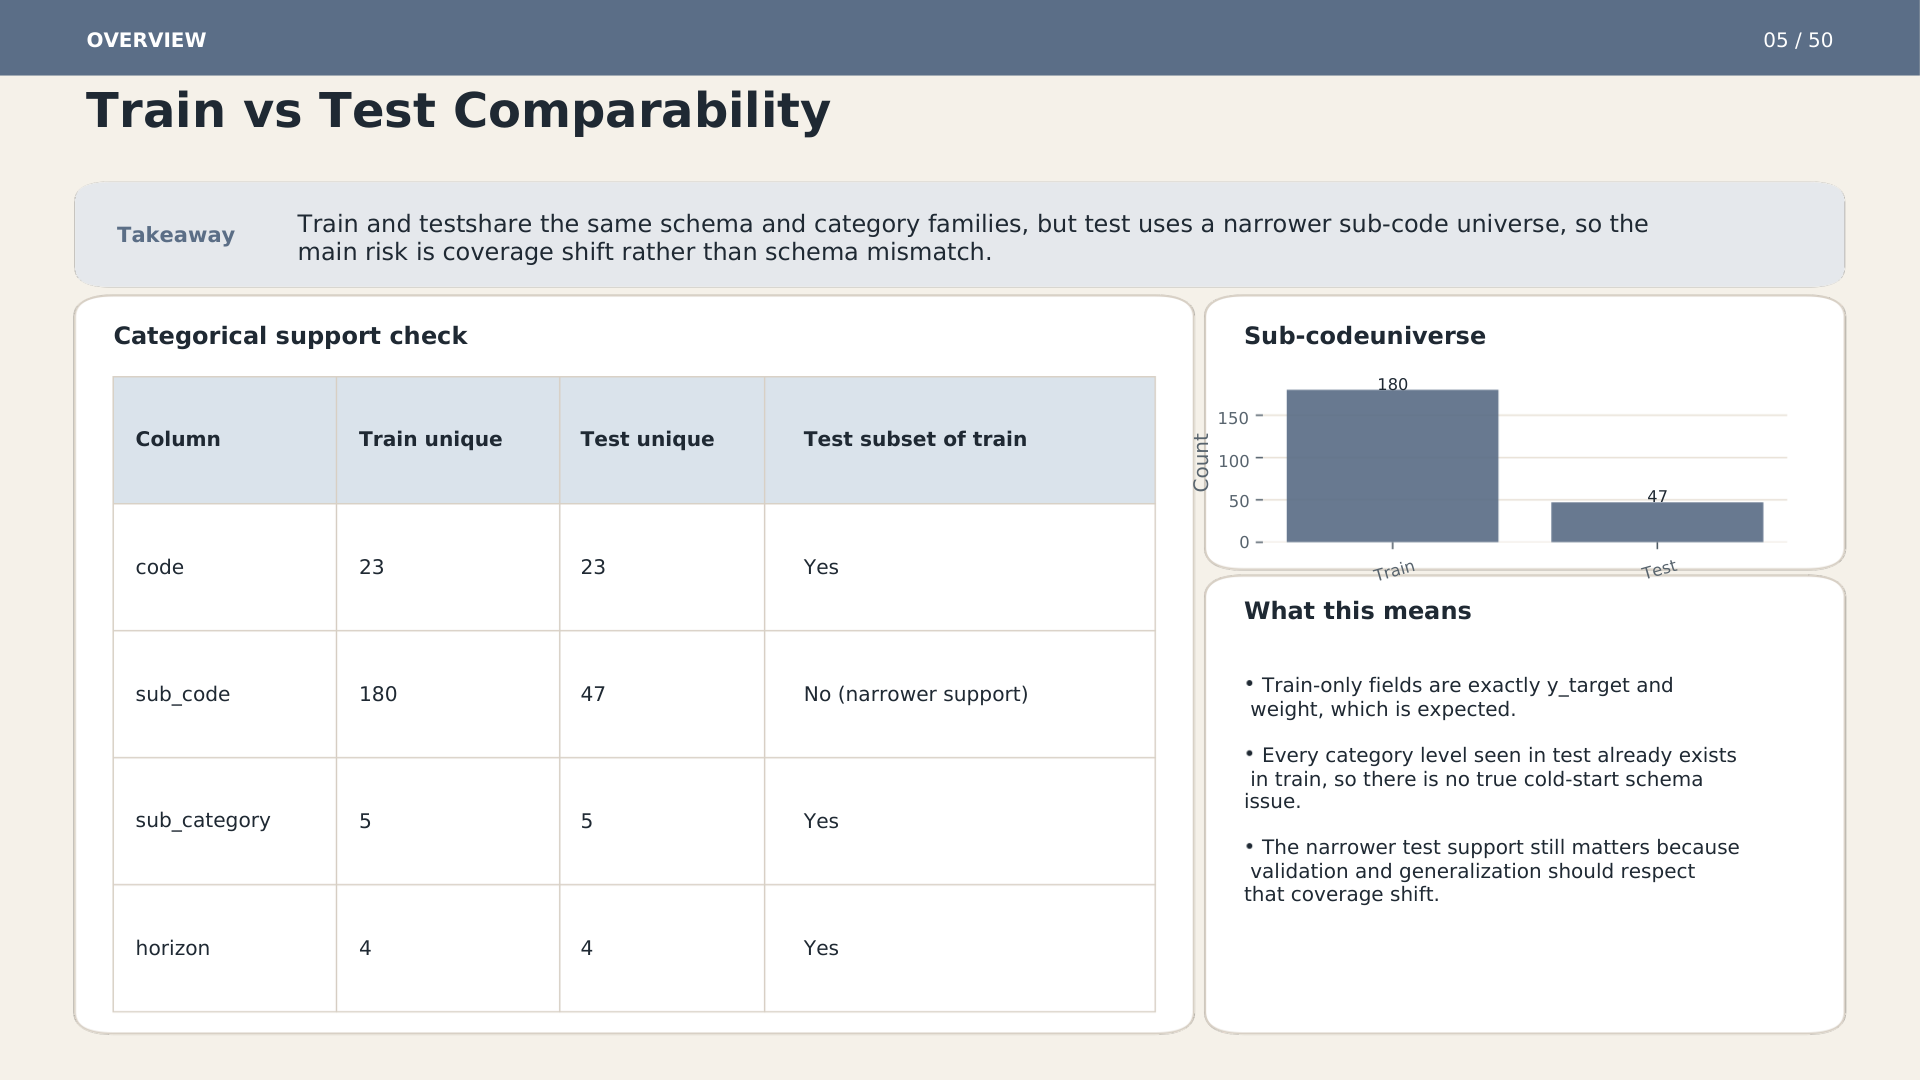
\includegraphics[width=0.95\textwidth]{figures/slide_05.png}
\caption{Train vs.~Test comparability analysis. The categorical support check reveals that train and test share the same schema and category families, but the test set uses a narrower sub-code universe (47 vs.~180), making coverage shift the primary risk.}
\label{fig:train_test_compare}
\end{figure}

\section{Competition Timeline}

\begin{table}[H]
\centering
\caption{Competition timeline.}
\begin{tabular}{ll}
\toprule
\textbf{Event} & \textbf{Date} \\
\midrule
Competition Start & January 9, 2026 \\
Competition Close & April 7, 2026 \\
Prize Pool & \$10,000 \\
\bottomrule
\end{tabular}
\end{table}

\section{Evaluation Metric: Weighted Skill Score}

Submissions are evaluated using a \textbf{Weighted Skill Score} defined as:

\begin{equation}
\text{Skill Score} = \sqrt{1 - \text{clip}_{[0,1]}\!\left(\frac{\sum_i w_i \cdot (y_i - \hat{y}_i)^2}{\sum_i w_i \cdot y_i^2}\right)}
\label{eq:skill_score}
\end{equation}

where:
\begin{itemize}
    \item $y_i$ is the true target value at observation $i$,
    \item $\hat{y}_i$ is the predicted value,
    \item $w_i$ is the observation-level weight,
    \item $\text{clip}_{[0,1]}(\cdot)$ clips the ratio to the interval $[0, 1]$.
\end{itemize}

\subsection{Metric Interpretation}

The denominator $\sum_i w_i \cdot y_i^2$ is precisely the weighted squared error of a \textbf{zero forecast} ($\hat{y}_i = 0$ for all $i$). Therefore:

\begin{itemize}
    \item A skill score of \textbf{0} means the model is no better than predicting zero everywhere.
    \item A skill score of \textbf{1} means perfect prediction.
    \item The square root compresses the scale, rewarding incremental improvements more at lower skill levels.
\end{itemize}

This metric design has several important implications:
\begin{enumerate}
    \item \textbf{Weights matter enormously.} The \texttt{weight} column determines how much each observation contributes to the aggregate score. As our EDA will show, weight concentration is extreme---the top 1\% of rows contribute approximately 65\% of the total weighted score.
    \item \textbf{Zero is a natural baseline.} The zero-forecast error appears explicitly in the denominator, making ``Zero'' a meaningful model to include in any leaderboard.
    \item \textbf{Unweighted metrics are misleading.} Any evaluation that ignores weights will rank models incorrectly with respect to the competition leaderboard.
\end{enumerate}

\section{Data Schema}

The competition provides two files in Apache Parquet format:

\begin{table}[H]
\centering
\caption{Competition data files.}
\begin{tabular}{lll}
\toprule
\textbf{File} & \textbf{Rows} & \textbf{Description} \\
\midrule
\texttt{train.parquet} & 5,337,414 & Training data with targets \\
\texttt{test.parquet} & --- & Test data (targets hidden) \\
\bottomrule
\end{tabular}
\end{table}

Each row in the training data contains:

\begin{table}[H]
\centering
\caption{Column schema for \texttt{train.parquet}.}
\label{tab:schema}
\begin{tabular}{lll}
\toprule
\textbf{Column} & \textbf{Type} & \textbf{Description} \\
\midrule
\texttt{code} & Categorical & Entity identifier (23 unique codes) \\
\texttt{sub\_code} & Categorical & Sub-entity identifier \\
\texttt{sub\_category} & Categorical & Category label \\
\texttt{horizon} & Integer & Forecast horizon (4 unique: 1, 5, 10, 22) \\
\texttt{ts\_index} & Integer & Temporal index (not calendar dates) \\
\texttt{y\_target} & Float & Target variable to forecast \\
\texttt{weight} & Float & Observation-level weight for scoring \\
\texttt{x0}--\texttt{x85} & Float & 86 anonymized predictor features \\
\bottomrule
\end{tabular}
\end{table}

\subsection{Panel Structure}

A unique time series is identified by the tuple \texttt{(code, sub\_code, sub\_category, horizon)}. The dataset contains \textbf{36,923 unique series} in total, with varying lengths. The integer-indexed \texttt{ts\_index} provides temporal ordering without revealing calendar information.

The four forecast horizons---1, 5, 10, and 22---suggest daily financial data with horizons corresponding to 1 day, 1 week, 2 weeks, and approximately 1 month of trading days.

\subsection{Anonymization}

All identifiers are anonymized (e.g., \texttt{MRV5UON2}, \texttt{KL66VIS3}, \texttt{V8BKY1IV}), and the 86 predictor features are labeled generically as \texttt{x0} through \texttt{x85}. This design prevents domain-specific shortcuts and forces participants to rely purely on statistical methodology.
